\documentclass[12pt]{article}
\usepackage{amsmath}
\usepackage{graphicx}
\usepackage{hyperref}
\usepackage[utf8]{inputenc}
\usepackage{geometry}
\usepackage{mathtools}
\usepackage{empheq}
\usepackage{listings}
\usepackage{xcolor}
\usepackage{authblk}
\usepackage{subcaption}
\usepackage{svg}
\usepackage{minted}


\definecolor{LightGray}{gray}{0.9}

\graphicspath{ {./assets/} }
\geometry{margin=0.5in}

\title{HW}
\date{}

\begin{document}

\begin{enumerate}

    \newpage
    \item Problem 1 (5.32)
    
    \begin{align*}
        & \sigma = 2 \\
        & \theta_{\text{rot}} = 2.07 \\
        q_{\text{rot}} &= \frac{T}{\sigma \theta_{\text{rot}}} = \frac{200}{2\cdot2.07} = 48.31 \\
    \end{align*}

    Plot:

    \[
       P_J = \frac{\left(2J+1\right)\exp\left(\frac{-J\left(J+1\right)\theta_{\text{rot}}}{T}\right)}{\sigma q_{\text{rot}}}  
    \]


    \begin{center}
        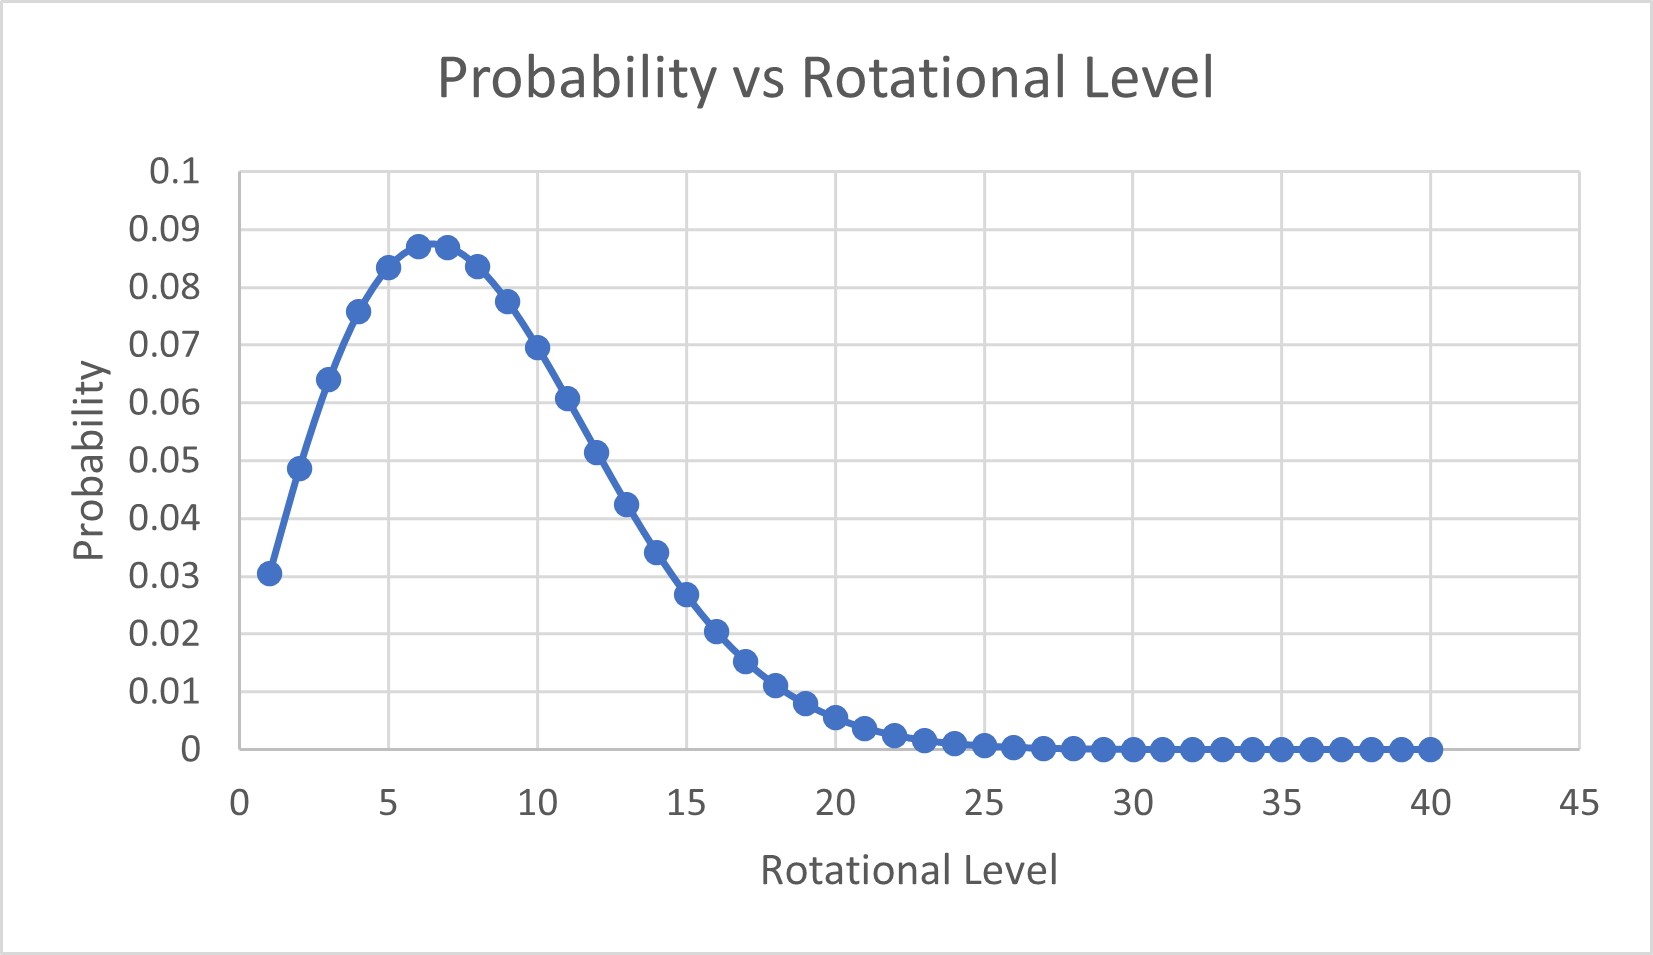
\includegraphics[width=0.8\textwidth]{assets/p1.png}
    \end{center}
    
    \newpage
    \item Problem 2 (5.33)
    
    \begin{align*}
        & \theta_{\text{vib}} = 308 \\
        q_{\text{vib}} &= \frac{1}{1-\exp\left(\frac{-\theta_{\text{vib}}}{T}\right)} = \frac{1}{1-\exp\left(\frac{-308}{1375}\right)} = 4.98
    \end{align*}

    Plot:

    \[
        P_n = \frac{\exp\left(\frac{-n\theta_{\text{vib}}}{T}\right)}{q_{\text{vib}}}  
    \]

    \begin{center}
        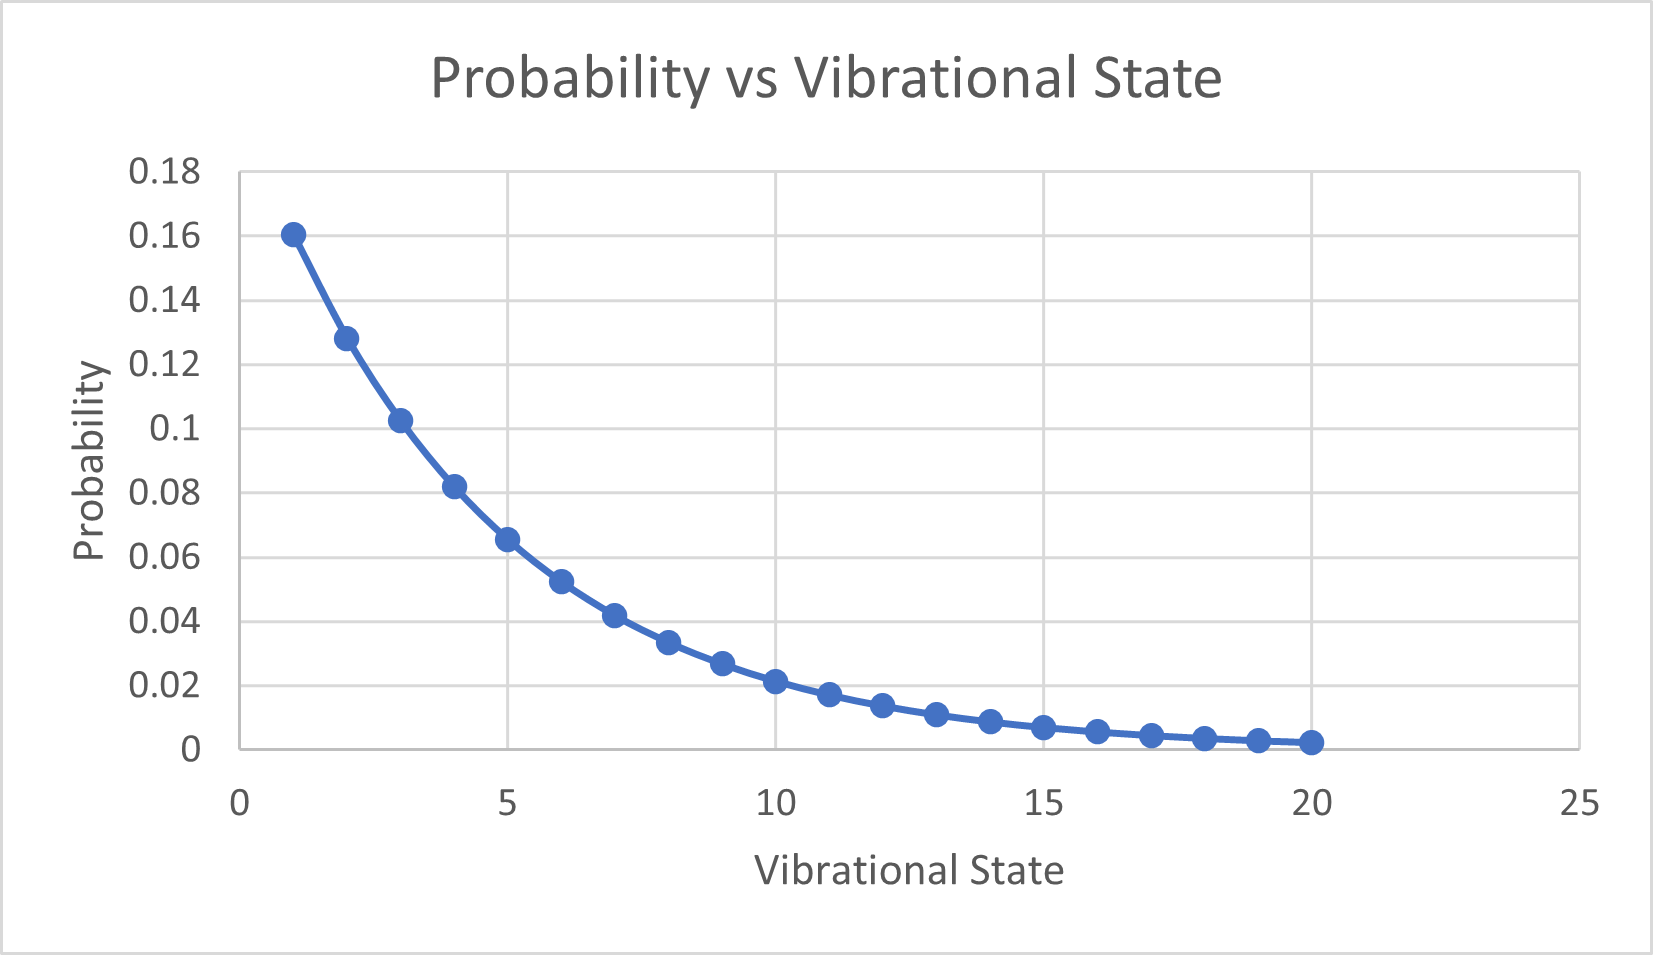
\includegraphics[width=0.8\textwidth]{assets/p2.png}
    \end{center}

    \newpage
    \item Problem 3 (5.34)
    
    \begin{align*}
        & T = 1375 \\
        & q_{\text{el, I}} = 4 \\
        & q_{\text{el, I$_2$}} = 1 \\
        & \theta_{\text{vib}} = 308 \\
        & \theta_{\text{rot}} = 0.0537 \\
        & D_0 = 148.8 \\
        & \sigma = 2 \\
        & \nu_{\text{I}_2} = -1 \\
        & \nu_{\text{I}} = 2 \\
        & P^\circ = 10^5 \\
        & k_B = 1.3807\cdot10^{-23} \\
        & h = 6.626\cdot10^{-34} \\
        & m_\text{I} = 2.107\cdot10^{-25} \\
        & m_{\text{I$_2$}} = 4.215\cdot10^{-25} \\
        \frac{k_B T}{P^\circ} &= \frac{1.3807\cdot10^{-23} \cdot 1375}{10^5} = 1.898\cdot10^{-25} \\
        q_{\text{rot}} &= \frac{T}{\sigma \theta_{\text{rot}}} = \frac{1375}{2\cdot0.0537} = 12802.6 \\
        q_{\text{vib}} &= \frac{1}{1-\exp\left(\frac{-\theta_{\text{vib}}}{T}\right)} = \frac{1}{1-\exp\left(\frac{-308}{1375}\right)} = 4.98 \\
        \exp\left(\frac{-\Delta U}{RT}\right) &= \exp\left(\frac{-148.8\cdot100}{8.314\cdot1375}\right) = 2.22\cdot10^{-6} \\
        K &= \frac{k_B T}{P^\circ} \cdot \frac{\left(\frac{2\pi k_B T}{h^2}\right)^{3/2} \cdot m_\text{I}^3 \cdot q_{\text{el, I}}^2}{m_{\text{I$_2$}}^{3/2} \cdot q_{\text{rot}} \cdot q_{\text{vib}} \cdot q_{\text{el, I$_2$}}} \cdot \exp\left(\frac{-\Delta U}{RT}\right) \\
        K &= 1.898\cdot10^{-25} \cdot \frac{\left(\frac{2\pi \cdot 1.3807\cdot10^{-23} \cdot 1375}{\left(6.626\cdot10^{-34}\right)^2}\right)^{3/2} \cdot \left(2.107\cdot10^{-25}\right)^3 \cdot 4^2}{\left(4.215\cdot10^{-25}\right)^{3/2} \cdot 12802.6 \cdot 4.98 \cdot 1} \cdot 2.22\cdot10^{-6} \\
        K &= 0.5128
    \end{align*}

    a.

    \begin{align*}
        x &= \left(\frac{K}{4\frac{P}{P^\circ}+K}\right)^{1/2} \\
        x &= \left(\frac{0.5128}{4\frac{0.1}{1}+0.5128}\right)^{1/2} \\
        \Aboxed{x &= 0.7495}
    \end{align*}

    b.

    \begin{align*}
        x &= \left(\frac{0.5128}{4\frac{1}{1}+0.5128}\right)^{1/2} \\
        \Aboxed{x &= 0.3371}
    \end{align*}

    c.

    \begin{align*}
        x &= \left(\frac{0.5128}{4\frac{0.01}{1}+0.5128}\right)^{1/2} \\
        \Aboxed{x &= 0.9631}
    \end{align*}
    
    \newpage
    \item Problem 4 (5.14)
    
    a.

    \begin{align*}
        W_{\text{A+B}} &= W_A W_B = 10^{26} \cdot 4 \cdot 10^{26} \\
        \Aboxed{W_{\text{A+B}} &= 4\cdot10^{52}}
    \end{align*}
    
    b.

    \begin{align*}
        S_i &= k_B \ln W_i \\
        S_A &= k_B \ln W_A = 1.3807\cdot10^{-23} \ln\left(10^{26}\right) \\ 
        \Aboxed{S_A &= 8.26\cdot10^{-22} \text{ J/K}} \\
        S_B &= k_B \ln W_B = 1.3807\cdot10^{-23} \ln\left(4\cdot10^{26}\right) \\ 
        \Aboxed{S_B &= 8.45\cdot10^{-22} \text{ J/K}} \\
        S_\text{A+B} &= S_A + S_B = 8.26\cdot10^{-22} + 8.45\cdot10^{-22} \\
        \Aboxed{S_A &= 1.67\cdot10^{-21} \text{ J/K}} \\
    \end{align*}
    
    \newpage
    \item Problem 5 (5.40)
    
    \begin{align*}
        R\ln\left(3\right) = 1.0986 R = 9.134 \text{ J/mol/K}
    \end{align*}

    The difference between spectroscopic and calorimetric entropies is that NDH$_2$ has 3 rotational arrangements based on the position of the D atom.

\end{enumerate}

\end{document}